% Chapter 4

\chapter{Introduction to Cross-platform Development with Xamarin} % Main chapter title

\label{Chapter4} % For referencing the chapter elsewhere, use \ref{Chapter1}

%----------------------------------------------------------------------------------------

%% Define some commands to keep the formatting separated from the content
% \newcommand{\keyword}[1]{\textbf{#1}}
% \newcommand{\tabhead}[1]{\textbf{#1}}
% \newcommand{\code}[1]{\texttt{#1}}
% \newcommand{\file}[1]{\texttt{\bfseries#1}}
% \newcommand{\option}[1]{\texttt{\itshape#1}}
 Xamarin offers sophisticated cross-platform support for the three major mobile platforms of iOS, Android, and Windows Phone.
 Applications can be written to share up to 90\% of their code, and our Xamarin.Mobile library offers a unified API to access common resources across all three platforms.
 This can significantly reduce both development costs and time to market for mobile developers that target the three most popular mobile platforms.

 %----------------------------------------------------------------------------------------


 \section{Introduction to Xamarin}

 When considering how to build iOS and Android applications, many people think that the native languages, Objective-C, Swift, and Java, are the only choice. However, over the past few years, an entire new ecosystem of platforms for building mobile applications has emerged.


 \paragraph{}
 Xamarin is unique in this space by offering a single language – C\#, class library, and runtime that works across all three mobile platforms of iOS, Android, and Windows Phone (Windows Phone’s native language is already C\#), while still compiling native (non-interpreted) applications that are performant enough even for demanding games.


 \paragraph{}
 Each of these platforms has a different feature set and each varies in its ability to write native applications – that is, applications that compile down to native code and that interop fluently with the underlying Java subsystem. For example, some platforms only allow apps to be built in HTML and JavaScript, whereas some are very low-level and only allow C/C++ code. Some platforms don’t even utilize the native control toolkit.

\paragraph{}
 Xamarin is unique in that it combines all of the power of the native platforms and adds a number of powerful features of its own, including:


 \begin{itemize}


   \item \textbf{ Complete Binding for the underlying SDKs:}   Xamarin contains bindings for nearly the entire underlying platform SDKs in both iOS and Android. Additionally, these bindings are strongly-typed, which means that they’re easy to navigate and use, and provide robust compile-time type checking and during development. This leads to fewer runtime errors and higher quality applications.

   \item \textbf{Objective-C, Java, C, and C++ Interop:}  Xamarin provides facilities for directly invoking Objective-C, Java, C, and C++ libraries, giving you the power to use a wide array of 3rd party code that has already been created. This lets you take advantage of existing iOS and Android libraries written in Objective-C, Java or C/C++. Additionally, Xamarin offers binding projects that allow you to easily bind native Objective-C and Java libraries using a declarative syntax.

   \item \textbf{Modern Language Constructs :}     Xamarin applications are written in C\#, a modern language that includes significant improvements over Objective-C and Java such as Dynamic Language Features , Functional Constructs such as Lambdas , LINQ , Parallel Programming features, sophisticated Generics , and more.

   \item \textbf{Amazing Base Class Library (BCL): }  Xamarin applications use the .NET BCL, a massive collection of classes that have comprehensive and streamlined features such as powerful XML, Database, Serialization, IO, String, and Networking support, just to name a few. Additionally, existing C\# code can be compiled for use in an applications, which provides access to thousands upon thousands of libraries that will let you do things that aren’t already covered in the BCL.

   \item \textbf{Modern Integrated Development Environment (IDE):}  Xamarin uses Xamarin Studio on Mac OS X and Visual Studio on Windows. These are both modern IDE’s that include features such as code auto completion, a sophisticated Project and Solution management system, a comprehensive project template library, integrated source control, and many others.

   \item \textbf{Mobile Cross Platform Support:}   Xamarin offers sophisticated cross-platform support for the three major mobile platforms of iOS, Android, and Windows Phone. Applications can be written to share up to 90\% of their code, and our Xamarin.Mobile library offers a unified API to access common resources across all three platforms. This can significantly reduce both development costs and time to market for mobile developers that target the three most popular mobile platforms.

 \end{itemize}


 %----------------------------------------------------------------------------------------






 %----------------------------------------------------------------------------------------


 \section{How Does Xamarin Work?}

 Xamarin offers two commercial products: Xamarin.iOS and Xamarin.Android.
 They’re both built on top of Mono, an open-source version of the .NET Framework based on the published .NET ECMA standards.
 Mono has been around almost as long as the .NET framework itself, and runs on nearly every imaginable platform including Linux, Unix, FreeBSD, and Mac OS X.

\paragraph{}
On iOS, Xamarin’s Ahead-of-Time ( AOT) Compiler compiles Xamarin.iOS applications directly to native ARM assembly code. On Android, Xamarin’s compiler compiles down to Intermediate Language ( IL), which is then Just-in-Time ( JIT) compiled to native assembly when the application launches.

In both cases, Xamarin applications utilize a runtime that automatically handles things such as memory allocation, garbage collection, underlying platform interop, etc.
 %----------------------------------------------------------------------------------------

%----------------------------------------------------------------------------------------

\section{Understanding the Xamarin Mobile Platform}
Welcome to this \LaTeX{} Thesis Template, a beautiful and easy to use template for writing a thesis using the \LaTeX{} typesetting system.

If you are writing a thesis (or will be in the future) and its subject is technical or mathematical (though it doesn't have to be), then creating it in \LaTeX{} is highly recommended as a way to make sure you can just get down to the essential writing without having to worry over formatting or wasting time arguing with your word processor.

\LaTeX{} is easily able to professionally typeset documents that run to hundreds or thousands of pages long. With simple mark-up commands, it automatically sets out the table of contents, margins, page headers and footers and keeps the formatting consistent and beautiful. One of its main strengths is the way it can easily typeset mathematics, even \emph{heavy} mathematics. Even if those equations are the most horribly twisted and most difficult mathematical problems that can only be solved on a super-computer, you can at least count on \LaTeX{} to make them look stunning.

%----------------------------------------------------------------------------------------

\section{Architecture}

A key tenet of building cross-platform apps is to create an architecture that lends itself to a maximization of code sharing across platforms. Adhering to the following Object Oriented Programming principles helps build a well-architected application:
 \begin{itemize}
\item \textbf{ Encapsulation:}     Ensuring that classes and even architectural layers only expose a minimal API that performs their required functions, and hides the implementation details. At a class level, this means that objects behave as ‘black boxes’ and that consuming code does not need to know how they accomplish their tasks. At an architectural level, it means implementing patterns like Façade that encourage a simplified API that orchestrates
\item \textbf{ Complete Binding for the underlying SDKs:}   more complex interactions on behalf of the code in more abstract layers. This means that the UI code (for example) should only be responsible for displaying screens and accepting user-input; and never interacting with the database directly. Similarly the data-access code should only read and write to the database, but never interact directly with buttons or labels.
\item \textbf{ Separation of Responsibilities:}     Ensure that each component (both at architectural and class level) has a clear and well-defined purpose. Each component should perform only its defined tasks and expose that functionality via an API that is accessible to the other classes that need to use it.
\item \textbf{ Polymorphism :}   Programming to an interface (or abstract class) that supports multiple implementations means that core code can be written and shared across platforms, while still interacting with platform-specific features.

\end{itemize}

\paragraph{}
The natural outcome is an application modeled after real world or abstract entities with separate logical layers. Separating code into layers make applications easier to understand, test and maintain. It is recommended that the code in each layer be physically separate (either in directories or even separate projects for very large applications) as well as logically separate (using namespaces).

\subsection{Typical Application Layers}


Throughout this document and the case studies we refer to the following six application layers:

\begin{itemize}
\item \textbf{Data Layer:}  – Non-volatile data persistence, likely to be a SQLite database but could be implemented with XML files or any other suitable mechanism.
\item \textbf{ Data Access Layer :} – Wrapper around the Data Layer that provides Create, Read, Update, Delete (CRUD) access to the data without exposing implementation details to the caller. For example, the DAL may contain SQL statements to query or update the data but the referencing code would not need to know this.
\item \textbf{ Business Layer:}  – (sometimes called the Business Logic Layer or BLL) contains business entity definitions (the Model) and business logic. Candidate for Business Façade pattern.
\item \textbf{Service Access Layer:}  – Used to access services in the cloud: from complex web services (REST, JSON, WCF) to simple retrieval of data and images from remote servers. Encapsulates the networking behavior and provides a simple API to be consumed by the Application and UI layers.
\item \textbf{ Application Layer:}  – Code that’s typically platform specific (not generally shared across platforms) or code that is specific to the application (not generally reusable). A good test of whether to place code in the Application Layer versus the UI Layer is (a) to determine whether the class has any actual display controls or (b) whether it could be shared between multiple screens or devices (eg. iPhone and iPad).
\item \textbf{ User Interface (UI) Layer:}  – The user-facing layer, contains screens, widgets and the controllers that manage them.

\end{itemize}

\paragraph{}
An application may not necessarily contain all layers – for example the Service Access Layer would not exist in an application that does not access network resources. A very simple application might merge the Data Layer and Data Access Layer because the operations are extremely basic.



\subsection{Common Mobile Software Patterns}

Patterns are an established way to capture recurring solutions to common problems. There are a few key patterns that are useful to understand in building maintainable/understandable mobile applications.
\begin{itemize}
\item \textbf{Model, View, ViewModel (MVVM):}  The Model-View-ViewModel pattern is popular with frameworks that support data-binding, such as Xamarin.Forms. It was popularized by XAML-enabled SDKs like Windows Presentation Foundation (WPF) and Silverlight; where the ViewModel acts as a go-between between the data (Model) and user interface (View) via data binding and commands.
\item \textbf{Model, View, Controller (MVC):}   A common and often misunderstood pattern, MVC is most often used when building User Interfaces and provides for a separation between the actual definition of a UI Screen (View), the engine behind it that handles interaction (Controller), and the data that populates it (Model). The model is actually a completely optional piece and therefore, the core of understanding this pattern lies in the View and Controller. MVC is a popular approach for iOS applications.
\item \textbf{Business Façade:}    AKA Manager Pattern, provides a simplified point of entry for complex work. For example, in a Task Tracking application, you might have a TaskManager class with methods such as GetAllTasks() , GetTask(taskID) , SaveTask (task) , etc. The TaskManager class provides a Façade to the inner workings of actually saving/retrieving of tasks objects.
\item \textbf{Singleton:}   The Singleton pattern provides for a way in which only a single instance of a particular object can ever exist. For example, when using SQLite in mobile applications, you only ever want one instance of the database. Using the Singleton pattern is a simple way to ensure this.
\item \textbf{Provider:}    A pattern coined by Microsoft (arguably similar to Strategy, or basic Dependency Injection) to encourage code re-use across Silverlight, WPF and WinForms applications. Shared code can be written against an interface or abstract class, and platform-specific concrete implementations are written and passed in when the code is used.
\item \textbf{Async:}   Not to be confused with the Async keyword, the Async pattern is used when long-running work needs to be executed without holding up the UI or current processing. In its simplest form, the Async pattern simply describes that long-running tasks should be kicked off in another thread (or similar thread abstraction such as a Task) while the current thread continues to process and listens for a response from the background process, and then updates the UI when data and or state is returned.

\end{itemize}


Each of the patterns will be examined in more detail as their practical use is illustrated in the case studies. Wikipedia has more detailed descriptions of the MVVM, MVC, Facade, Singleton, Strategy and Provider patterns (and of Design Patterns generally).



%----------------------------------------------------------------------------------------
\section{Setting Up A Xamarin Cross Platform Solution}

Regardless of what platforms are being used, Xamarin projects all use the same solution file format (the Visual Studio .sln file format).
Solutions can be shared across development environments, even when individual projects cannot be loaded (such as a Windows project in Xamarin Studio).

When creating a new cross platform application, the first step is to create a blank solution.
This section what happens next: setting up the projects for building cross platform mobile apps

\subsection{Code Sharing Options}
\LaTeX{} is not a \textsc{wysiwyg} (What You See is What You Get) program, unlike word processors such as Microsoft Word or Apple's Pages. Instead, a document written for \LaTeX{} is actually a simple, plain text file that contains \emph{no formatting}. You tell \LaTeX{} how you want the formatting in the finished document by writing in simple commands amongst the text, for example, if I want to use \emph{italic text for emphasis}, I write the \verb|\emph{text}| command and put the text I want in italics in between the curly braces. This means that \LaTeX{} is a \enquote{mark-up} language, very much like HTML.

\subsection{Portable Class Libraries}

Historically a .NET project file (and the resulting assembly) has been targeted to a specific framework version. This prevents the project or the assembly being shared by different frameworks.

A Portable Class Library (PCL) is a special type of project that can be used across disparate CLI platforms such as Xamarin.iOS and Xamarin.Android, as well as WPF, Universal Windows Platform, and Xbox. The library can only utilize a subset of the complete .NET framework, limited by the platforms being targeted.

\subsection{Shared Projects}
The simplest approach to sharing code files is use a Shared Project.

This method allows you to share the same code across different platform projects, and use compiler directives to include different, platform-specific code paths.

Shared Projects (also sometimes called Shared Asset Projects) let you write code that is shared between multiple target projects including Xamarin applications.

They support compiler directives so that you can conditionally include platform-specific code to be compiled into a subset of the projects that are referencing the Shared Project. There is also IDE support to help manage the compiler directives and visualize how the code will look in each application.

If you have used file-linking in the past to share code between projects, Shared Projects works in a similar way but with much improved IDE support.

\begin{figure}[th]
\centering
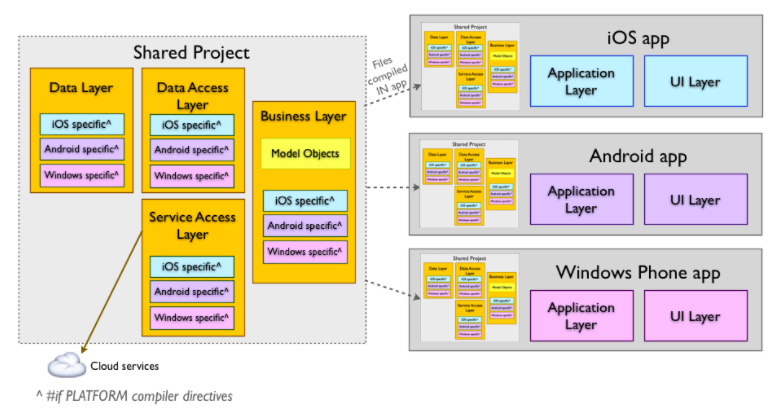
\includegraphics[width=\textwidth] {Figures/SharedProjects}

\caption[Shared Projects architecture]{Shared Projects application architecture.}
\label{fig:SharedProjectsarchitecture}
\end{figure}
% referance add

Shared Project Example


\subsection{.NET Standard}

Introduced in 2016, .NET Standard projects provide an easy way to share code across platforms, producing assemblies that can be used across Windows, Xamarin platforms (iOS, Android, Mac), and Linux.

.NET Standard libraries can be created and used like PCLs, except that the APIs available in each version (from 1.0 to 1.6) are more easily discovered and each version is backwards-compatible with lower version numbers.



\subsection{Core Project}
Shared code projects should only reference assemblies that are available across all platforms – ie. the common framework namespaces like System, System.Core and System.Xml.

Shared projects should implement as much non-UI functionality as is possible, which could include the following layers:
\begin{itemize}

\item \textbf{ Data Layer :}  Code that takes care of physical data storage eg. SQLite-NET, an alternative database like Realm.io or even XML files. The data layer classes are normally only used by the data access layer.
\item \textbf{Data Access Layer:}   Defines an API that supports the required data operations for the application’s functionality, such as methods to access lists of data, individual data items and also
\item \textbf{Service Access Layer :}   An optional layer to provide cloud services to the application. Contains code that accesses remote network resources (web services, image downloads, etc) and possibly caching of the results.
\item \textbf{Business Layer:}  Definition of the Model classes and the Façade or Manager classes that expose functionality to the platform-specific applications.


\end{itemize}


\subsection{Platform-Specific Application Projects}
Platform-specific projects must reference the assemblies required to bind to each platform’s SDK (Xamarin.iOS, Xamarin.Android, Xamarin.Mac, or Windows) as well as the Core shared code project.

The platform-specific projects should implement:
\begin{itemize}

\item \textbf{ Application Layer:} Platform specific functionality and binding/conversion between the Business Layer objects and the user interface.
\item \textbf{ User Interface Layer:} Screens, custom user-interface controls, presentation of validation logic.
\end{itemize}

\begin{figure}[th]
\centering
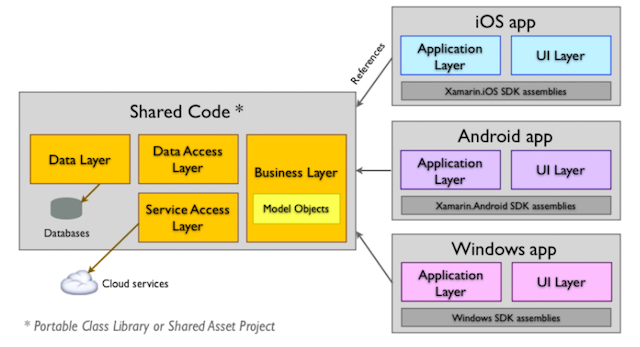
\includegraphics[width=\textwidth] {Figures/Xamarin_architecture}

\caption[architecture]{application architecture.}
\label{fig:architecture}
\end{figure}

% referance add


%----------------------------------------------------------------------------------------

\section{Dealing with Multiple Platforms}

If you are familiar with \LaTeX{}, then you should explore the directory structure of the template and then proceed to place your own information into the \emph{THESIS INFORMATION} block of the \file{main.tex} file. You can then modify the rest of this file to your unique specifications based on your degree/university. Section \ref{FillingFile} on page \pageref{FillingFile} will help you do this. Make sure you also read section \ref{ThesisConventions} about thesis conventions to get the most out of this template.

If you are new to \LaTeX{} it is recommended that you carry on reading through the rest of the information in this document.

Before you begin using this template you should ensure that its style complies with the thesis style guidelines imposed by your institution. In most cases this template style and layout will be suitable. If it is not, it may only require a small change to bring the template in line with your institution's recommendations. These modifications will need to be done on the \file{MastersDoctoralThesis.cls} file.

%----------------------------------------------------------------------------------------
\section{Practical Code Sharing Strategies}

If you are familiar with \LaTeX{}, then you should explore the directory structure of the template and then proceed to place your own information into the \emph{THESIS INFORMATION} block of the \file{main.tex} file. You can then modify the rest of this file to your unique specifications based on your degree/university. Section \ref{FillingFile} on page \pageref{FillingFile} will help you do this. Make sure you also read section \ref{ThesisConventions} about thesis conventions to get the most out of this template.

If you are new to \LaTeX{} it is recommended that you carry on reading through the rest of the information in this document.

Before you begin using this template you should ensure that its style complies with the thesis style guidelines imposed by your institution. In most cases this template style and layout will be suitable. If it is not, it may only require a small change to bring the template in line with your institution's recommendations. These modifications will need to be done on the \file{MastersDoctoralThesis.cls} file.

%----------------------------------------------------------------------------------------
\section{Dealing with Multiple Platforms}

If you are familiar with \LaTeX{}, then you should explore the directory structure of the template and then proceed to place your own information into the \emph{THESIS INFORMATION} block of the \file{main.tex} file. You can then modify the rest of this file to your unique specifications based on your degree/university. Section \ref{FillingFile} on page \pageref{FillingFile} will help you do this. Make sure you also read section \ref{ThesisConventions} about thesis conventions to get the most out of this template.

If you are new to \LaTeX{} it is recommended that you carry on reading through the rest of the information in this document.

Before you begin using this template you should ensure that its style complies with the thesis style guidelines imposed by your institution. In most cases this template style and layout will be suitable. If it is not, it may only require a small change to bring the template in line with your institution's recommendations. These modifications will need to be done on the \file{MastersDoctoralThesis.cls} file.


%----------------------------------------------------------------------------------------
\section{Cross-Platform User Interfaces with Xamarin.Forms}

If you are familiar with \LaTeX{}, then you should explore the directory structure of the template and then proceed to place your own information into the \emph{THESIS INFORMATION} block of the \file{main.tex} file. You can then modify the rest of this file to your unique specifications based on your degree/university. Section \ref{FillingFile} on page \pageref{FillingFile} will help you do this. Make sure you also read section \ref{ThesisConventions} about thesis conventions to get the most out of this template.

\subsection{eXtensible Application Markup Language (XAML)}
If you are new to \LaTeX{} it is recommended that you carry on reading through the rest of the information in this document.

Before you begin using this template you should ensure that its style complies with the thesis style guidelines imposed by your institution. In most cases this template style and layout will be suitable. If it is not, it may only require a small change to bring the template in line with your institution's recommendations. These modifications will need to be done on the \file{MastersDoctoralThesis.cls} file.




%----------------------------------------------------------------------------------------
\section{Testing and App Store Approvals}

Many apps (even Android apps, on some stores) will have to pass an approval process before they are published; so testing is critical to ensure your app reaches the market (let alone succeeds with your customers). Testing can take many forms, from developer-level unit testing to managing beta testing across a wide variety of hardware.




\subsection{Test on All Platforms}

TThere are slight differences between what .NET supports on Windows phone, tablet, and desktop devices, as well as limitations on iOS that prevent dynamic code to be generated on the fly. Either plan on testing the code on multiple platforms as you develop it, or schedule time to refactor and update the model part of your application at the end of the project.

It is always good practice to use the simulator/emulator to test multiple versions of the operating system and also different device capabilities/configurations.

You should also test on as many different physical hardware devices as you can.


Devices in cloud
The mobile phone and tablet ecosystem is growing all the time, making it impossible to test on the ever-increasing number of devices available. To solve this problem a number of services offer the ability to remotely control many different devices so that applications can be installed and tested without needing to directly invest in lots of hardware.

Xamarin Test Cloud offers an easy way to test iOS and Android appliations on hundreds of different devices.


\subsection{Test Management}

When testing applications within your organization or managing a beta program with external users, there are two challenges:

Distribution – Managing the provisioning process (especially for iOS devices) and getting updated versions of software to the testers.
Feedback – Collecting information about application usage, and detailed information on any errors that may occur.
There are a number of services help to address these issues, by providing infrastructure that is built into your application to collect and report on usage and errors, and also streamlining the provisioning process to help sign-up and manage testers and their devices.

The Xamarin Insights Preview offers a solution to the second part of this issue, providing crash reporting and sophisticated application usage information.


\subsection{Test Automation}
Xamarin UITest can be used to create automated user interface test scripts that can be run locally or uploaded to Test Cloud.


\subsection{Unit Testing}

Touch.Unit
Xamarin.iOS includes a unit-testing framework called Touch.Unit which follows the JUnit/NUnit style writing tests.

Refer to our Unit Testing with Xamarin.iOS documentation for details on writing tests and running Touch.Unit.


Andr.Unit
There is an open-source equivalent of Touch.Unit for Android called Andr.Unit. You can download it from github and read about the tool on @spouliot's blog.


Windows Phone
Here are some links to help setup unit testing for Windows Phone:
